\documentclass[10pt,a4paper]{article}
\usepackage[utf8]{inputenc}
\usepackage[T1]{fontenc}
\usepackage{lmodern}
\usepackage[margin=1.5cm, top=1.4cm, bottom=1.4cm]{geometry}
\usepackage{hyperref}
\usepackage{enumitem}
\usepackage{titlesec}
\usepackage{xcolor}
\usepackage{graphicx}

\definecolor{accent}{HTML}{00686E}
\hypersetup{colorlinks=true, urlcolor=accent, linkcolor=accent}
\pagenumbering{arabic}
\setlength{\parindent}{0pt}

\titleformat{\section}{\large\bfseries\color{accent}}{}{0em}{}[\vspace{-0.6em}\rule{\textwidth}{0.8pt}]
\titlespacing{\section}{0pt}{7pt}{4pt}

\newcommand{\role}[4]{%
  \textbf{#1} \hfill \textbf{#2}\\[1pt]%
  \textit{#3} \hfill \textit{#4}\\[2pt]%
}
\setlist[itemize]{leftmargin=1.2em, itemsep=1.5pt, topsep=2pt, parsep=0pt}

\begin{document}

% ================= HEADER =================
\begin{minipage}[c]{0.80\textwidth}
  {\Huge\bfseries Prabhavit Gupta}\\[3pt]
  {\color{accent}\large Lead Product Engineer: Python, SQL, RAG \& AI Data Infrastructure}\\[6pt]
  {\footnotesize +39 351 610 7807 ~$\vert$~
  \href{mailto:prabhavitg@gmail.com}{prabhavitg@gmail.com} ~$\vert$~
  \href{https://www.linkedin.com/in/prabhavit/}{linkedin.com/in/prabhavit} ~$\vert$~
  \href{https://github.com/prab-gupta}{github.com/prab-gupta} ~$\vert$~
  Venice, Italy (CET Time Zone / EU Permanent Resident)}
\end{minipage}\hfill
\begin{minipage}[c]{0.18\textwidth}
  \raggedleft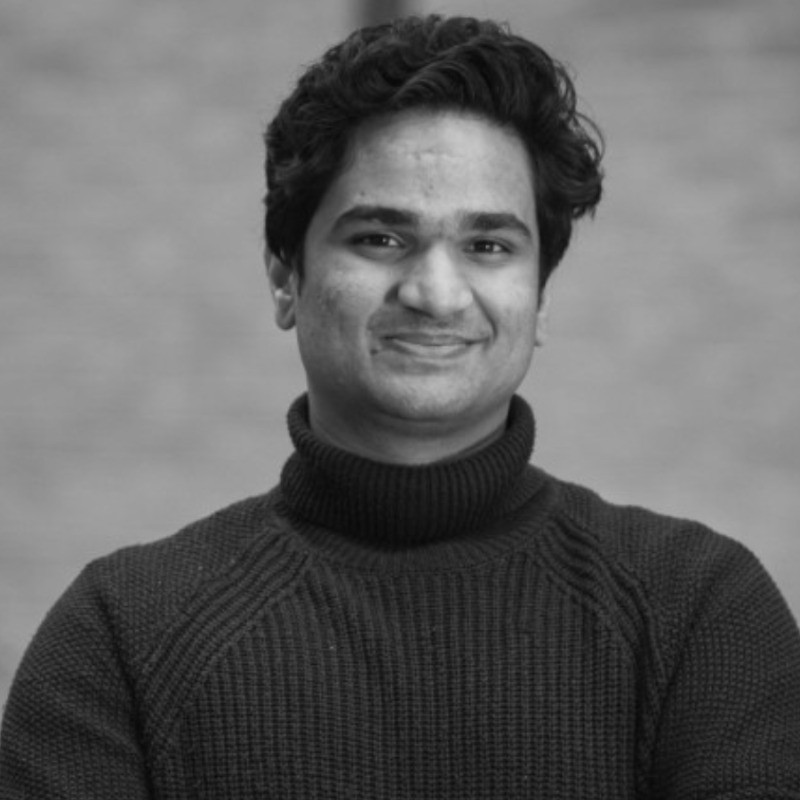
\includegraphics[width=2.0cm]{photo.jpg}
\end{minipage}
\vspace{-2pt}

% ================= SUMMARY =================
\section{Summary}
Lead Product Engineer and Software Architect with 3 years of commercial experience taking complex data and AI systems from 0 to 1 in production. Proven track record turning proprietary data assets into reliable, searchable intelligence layers combining Python, SQL data infrastructure, Retrieval-Augmented Generation (RAG), and TypeScript services. Experienced owning end-to-end technical delivery, designing clean API contracts, and establishing automated testing and evaluation standards. Based in Venice, Italy (CET time zone) with an EU Long-Term Residence Permit (permanent unrestricted EU work authorization, no sponsorship required); available immediately for full-time EU remote roles.

% ================= TECHNICAL EXPERTISE =================
\section{Technical Expertise}
\begin{itemize}
  \item \textbf{Data Infrastructure \& SQL:} PostgreSQL (relational schema design, complex analytical SQL, JSONB indexing, connection pooling), Redis task queues, ETL data ingestion pipelines.
  \item \textbf{AI Engineering \& RAG:} Retrieval-Augmented Generation, vector embeddings, hybrid semantic and keyword search, context injection, LangChain, tool calling, model evaluation harnesses.
  \item \textbf{Backend \& Full-Stack Development:} Python (FastAPI, asyncio, pandas, NumPy, Pydantic), TypeScript, Node.js, Next.js, RESTful microservices, structured JSON validation.
  \item \textbf{Architecture \& 0-to-1 Ownership:} Technical discovery, modular platform architecture, schema migrations, asynchronous messaging, rate limiting, and observability.
  \item \textbf{DevOps \& Testing:} Docker containerization, AWS/GCP cloud services, CI/CD pipeline automation, GitOps, automated regression and contract testing with Playwright.
  \item \textbf{Languages \& Authorization:} English (C1 Professional, fluent), Hindi (Native), Italian (Conversational). EU Long-Term Residence Permit (unrestricted EU work authorization across all EU member states, no sponsorship required).
\end{itemize}

% ================= EXPERIENCE =================
\section{Experience}

\role{\href{https://flowspace.co}{FlowSpace.co}}{Mar 2024 - Aug 2026}{Lead Developer \& AI Systems Architect}{London, UK (remote)}
\begin{itemize}
  \item Led 0-to-1 product engineering of customer-facing AI and data retrieval platforms for a marketplace serving 4,500+ active enterprise users across Europe.
  \item Architected high-performance Python (FastAPI) and PostgreSQL data pipelines, converting raw multi-source datasets into structured, searchable intelligence assets.
  \item Implemented production RAG systems with hybrid vector search, dynamic context window management, and automated evaluation harnesses measuring precision and recall.
  \item Designed asynchronous task processing with Redis, decoupling resource-intensive data indexing from synchronous client API requests.
  \item Led full-stack TypeScript and Node.js modernization, ensuring high performance, zero downtime, and seamless data synchronization.
  \item Authored core technical documentation, database schemas, and CI/CD automated test suites with Playwright, ensuring platform stability across rapid release cycles.
\end{itemize}

\role{Urlink}{Apr 2025 - Jul 2025}{Project Manager \& Solutions Developer (Freelance)}{Barcelona, Spain (remote)}
\begin{itemize}
  \item Led technical discovery, solution architecture, and delivery of custom full-stack web platforms and automated data synchronization services.
  \item Built ETL data ingestion pipelines connecting third-party APIs to PostgreSQL databases, maintaining strict data freshness and provenance.
  \item Created interactive prototypes and automated validation checks to verify functional specifications prior to production delivery.
\end{itemize}

\role{Independent Technical Consultant}{Aug 2023 - Feb 2024}{AI Automation \& Integration Developer}{Venice, Italy}
\begin{itemize}
  \item Developed custom Python utilities, SQL data models, and LLM integrations for European clients, automating document parsing and classification.
  \item Built robust data validation routines ensuring incoming unstructured web content conformed to rigorous relational database schemas.
  \item Authored technical architecture specifications, API documentation, and deployment guides for client engineering teams.
\end{itemize}

% ================= EDUCATION =================
\section{Education}
\role{Ca' Foscari University of Venice}{2020 - 2024}{BA in Philosophy, International Studies and Economics}{Venice, Italy}
\begin{itemize}
  \item Rigorous training in formal logic, analytical problem solving, systems analysis, and macroeconomic decision models.
\end{itemize}

\end{document}
